%
% einleitung.tex -- Beispiel-File für die Einleitung
%
% (c) 2020 Prof Dr Andreas Müller, Hochschule Rapperswil
%
% !TEX root = ../../buch.tex
% !TEX encoding = UTF-8
%

\section{Einleitung}
In diesem Kapiteln wird beschrieben, was unter zweidimensionaler Elektrostatik verstanden wird, welche physikalischen und mathematischen Gesetze ihr zugrunde liegen und wie diese zur Berechnung und Darstellung elektrostatischer Felder eingesetzt werden können.
Ausgehend vom Coulomb-Gesetz werden das elektrische Feld und das elektrische Potential eingeführt und deren Zusammenhang beschrieben. 
Dabei wird betrachtet, wie sich elektrische Felder und Potentiale im zweidimensionalen Raum darstellen lassen und welche Eigenschaften ihre Feld- und Äquipotentiallinien haben.
Weiter wird erörtert, wie diese Grössen mithilfe komplexer Funktionen beschrieben werden können. 
Dies dient als mathematische Grundlage, um elektrostatische Probleme nicht nur für einfache Geometrien wie den Kreis, sondern auch für kompliziertere Formen zu beschreiben.
Es wird der Riemannsche Abbildungssatz vorgestellt und erläutert, wie wie verschiedene Geometrien auf einfachere Gebiete abgebildet werden, für welche das elektrische Feld und das Potential bereits bekannt sind. 
Am Beispiel des Kreises und später mithilfe der Schwarz-Christoffel-Transformation wird gezeigt, wie dieses Prinzip auf verschiedene Geometrien angewendet werden kann.

Bevor wir in das Kapitel einsteigen, mögen einige Beispiel zur Anschauung dienen: 
Elektrostatik wird für uns Menschen erfahrbar, wenn es zu Ladungstrennungen kommt.
Blitze, klebende Styroporkügelchen und und als Sonderbeispiel Van de Graaff Bandgeneratoren --- Grundlage für diese physikalischen Phänomene ist folgendes Prinzip:
Gleichartige Ladungen stossen sich ab, ungleichartige Ladungen ziehen sich an.
Beispielsweise wenn wir einen synthetischen Pullover über den Kopf ziehen und dabei ein Knistern hören. Berühren wir dann einen anderen (geerdeten) Menschen, funkt es.
Ein kurzes Zwicken beweist die unsichtbare elektrostatische Aufladung, die durch Reibung des Pullovers erzeugt worden ist.
Als Fachpersonen im Bereich der Elektrotechnik haben wir häufig Bauteile in der Hand, die wir vor elektrostatischer Entladung (ESD) schützen müssen.
Zum Schutz solcher empfindlicher Bauteile tragen wir daher geerdete Armbänder, was Ladungstrennung, welche zu ESD führt, verhindert. 

Um elektrostatische Aufladung zu demonstrieren, wird eine (langhaarige) Versuchsperson daher zuallererst auf ein isoliertes Podest gestellt.
Ladung, die durch den von Robert Van de Graaff 1929 erfundenen Generator auf eine Metallkugel gebracht wird, gelangt mittels Berührung der Handflächen auf die Versuchsperson.
%\textcolor{red}{TODO Foto Versuchsperson mit Feldlinien eingezeichnet}
Der Van de Graaff Generator nutzt die mechanische Reibung eines Gummibandes, um gleichartige Ladungsträger auf einer Metallkugel abzuladen, welche sich anschliessend durch Influenz auf der ganzen Oberfläche verteilen.
Es spielt dabei keine Rolle, ob die Ladungsträger positiv oder negativ sind.
Die Ladungen wandern auf die Versuchsperson, und da sie sich abstossen, entsteht eine kleine Kraft.
Diese reicht bei genügend trockener Luft aus, um die Haare der Versuchsperson zu Berge stehen zu lassen.
Trotz seines tiefen Wirkungsgrades kommt der Van de Graaff Generator zur Erzeugung hoher Gleichspannungen als Teilchenbeschleuniger zum Einsatz \cite{elektro:lexikon}.

% In diesem Kapitel werden die Zusammenhänge zwischen Elektrostatik und Geometrie beschrieben. 
% Die Geometrie wird auf zwei Dimensionen reduziert, was zu Vereinfachungen führt.
% Die prominenteste Vereinfachung ist, dass von den vier Maxwell-Gleichungen nur noch eine relevant ist, nämlich die Laplace Gleichung (\ref{elektro:equation:laplace}) für das Potential. 
% Der Fokus liegt auf dem Zusammenhang zwischen elektrischen Feldlinien und Äquipotentiallinien im zweidimensionalen Raum.
% Feldlinien und Potential werden als komplexe Funktionen interpretiert und über komplexe Abbildungen miteinander verknüpft.
% Wie das funktioniert, wird anhand von vielen Beispielen in diesem Kapitel erklärt, bewiesen und veranschaulicht. 


\section{Grundlagen der Elektrostatik\label{elektro:section:EFeld}}
\kopfrechts{Grundlagen der Elektrostatik}
Das Begriff Elektrostatik enthält zwei grundlegende Begriffe: Elektrizität und Statik. 
Es fliesst aber kein Strom, es werden ausschliesslich ruhende elektrische Ladungsträger betrachtet.
In unseren Anwendungen verteilen sich diese Ladungen auf der Oberfläche von leitenden Körpern, bis die Kräfte zwischen den Ladungen einen stabilen Zustand erreicht haben, und still stehen bleiben.
Dann spricht man von Elektrostatik, denn die Ladungen bewegen sich nicht mehr, sie sind statisch. Wird nach der Zeit abgeleitet, um die Änderung über die Zeit zu sehen, so ist die Ableitung
$\frac{\partial \vec{E}}{\partial t} = 0$
gleich Null. 

\subsection{Vektor- und Skalarfeld, Quellenfeld und Homogenität
\label{elektro:subsection:VektorSkalar}}
Das \textbf{elektrische Feld} ist ein Vektorfeld.
Das bedeutet, jedem Punkt im Raum wird ein Vektor mit einem Betrag und einer Richtung der elektrischen Feldstärke zugeordnet. 
Die Länge des Vektors zeigt, wie stark das elektrische Feld an diesem Punkt ist. 
Seine Richtung ist diejenige Richtung, in die eine Probeladung bewegt wird, wenn sie an diesem Punkt platziert würde.
Eine Probeladung ist eine Ladung, die so klein ist, dass sie das Feld nicht beeinflusst.
Sie ist nur da um die Stärke des Feldes zu messen, ist also nur ein Werkzeug und keine physische Ladung.
Das \textbf{Potentialfeld} ist ein Skalarfeld.
Jedem Punkt im Raum wird nur der Betrag, also nur die Stärke des Potentials zugeordnet, aber keine Richtung.
Diese Stärke wird in Volt angegeben, das ist die definiere Einheit für das Potential.

Elektrostatische Felder sind Quellenfelder, das bedeutet, es gibt einen Punkt, von dem alle Feldlinien ausgehen oder auf den alle Feldlinien zulaufen. 
Es hat keine Wirbel, die Pfeile sind somit nicht in eine Richtung gebogen, sondern immer gerade.
Es ergeben sich also keine geschlossenen Feldlinien, die in sich selbst enden (wie es zum Beispiel beim Magnetfeld der Fall ist).
Die Feldlinien des elektrostatischen Felds beginnen immer auf positiven Ladungen und enden auf negativen. 
Die Feldlinien können sich aber im Unendlichen schliessen, somit laufen die Feldlinien einfach radial bis ins Unendliche.

Verlaufen die Feldlinien parallel, spricht man von einem homogenen Feld, ansonsten von einem inhomogenen Feld.
Das Feld zwischen zwei parallelen Kondensatorplatten beispielsweise ist homogen, was die mathematische Berechnung erheblich erleichtert. 

\subsection{Das Coulomb-Gesetz
\label{elektro:subsection:Coulomb}}
Das Coulomb-Gesetz
\begin{equation}
	\vec{F} = \frac{Q_1 Q_2}{4\pi\varepsilon_0 R^{2}}\hat{R}
	\label{equation:Coulomb}
\end{equation}
beschreibt die Kraft, die zwei ruhende Punktladungen aufeinander ausüben.
Eine Punktladung ist eine punktsymmetrische Ladung ohne räumliche Ausdehnung.
In der Praxis ist das Coulomb-Gesetz nur gültig, wenn der Abstand zwischen den beiden Ladungen viel grösser ist als die Ausdehnung der Ladungen selbst.
Ist dies nicht der Fall, werden sich andere physikalische Effekte bemerkbar machen, die das Coulomb-Gesetz nicht berücksichtigt.
Die Coulomb-Kraft hängt von der Grösse der jeweiligen Ladung $Q_1$ und $Q_2$ ab.
Werden die Ladungen grösser, so nimmt auch die Kraft zu.
Der Abstand zwischen den beiden Ladungen ist der bestimmende Faktor, da die Kraft mit dem Quadrat des Abstands $R$ zwischen den Ladungen abnimmt.
$\vec{R} = R \cdot \hat{R}$ ist der Distanzvektor zwischen den Ladungen und muss immer vom Ort der Ursache auf den Ort der Wirkung zeigen, damit die resultierenden Kräfte die korrekte Richtung aufweisen.
$\hat{R}$ ist in der Elektrotechnik der Einheitsvektor der Länge 1 und Richtung von $\vec{R}$.
Liegt einer der Punkte im Ursprung wird die Variable $r$ verwendet, dies ist wichtig für das Verstehen der später hergeleiteten Formeln.
Die beiden Komponenten des Vektors sind der Betrag $R$ und die Richtung $\hat{R}$, diese werden in der Formel \eqref{equation:Coulomb} separat verwendet.
Weitere wichtige Definitionen:
\begin{itemize}
	\item Das Coulomb-Gesetz gilt für Distanzen zwischen $10^{-16}$ und $10^{8}$ Metern. 
	\item Für $R = 0$ ist es nicht definiert. 
	\item $\varepsilon_0$ ist die elektrische Permittivität des Vakuums und beträgt ungefähr 8.854 pF/m. 
\end{itemize}

\subsection{Das elektrische Feld}
Im ersten Abschnitt \ref{elektro:section:EFeld} wurde das elektrische Feld als Vektorfeld definiert.
Es geht nun darum, das E-Feld auch mathematisch zu definieren.
Das elektrische Feld und die Coulomb-Kraft sind über die Normierung auf die Probeladung q
\begin{equation}
	\vec{E} = \frac{\vec{F}}{q} = \frac{\text{Kraft}}{\text{Probeladung}} = \frac{Q}{4\pi\varepsilon_0 r^{2}}\hat{r}
	\label{elektro:equation:EFeld}
\end{equation}
\begin{figure}
	\centering
	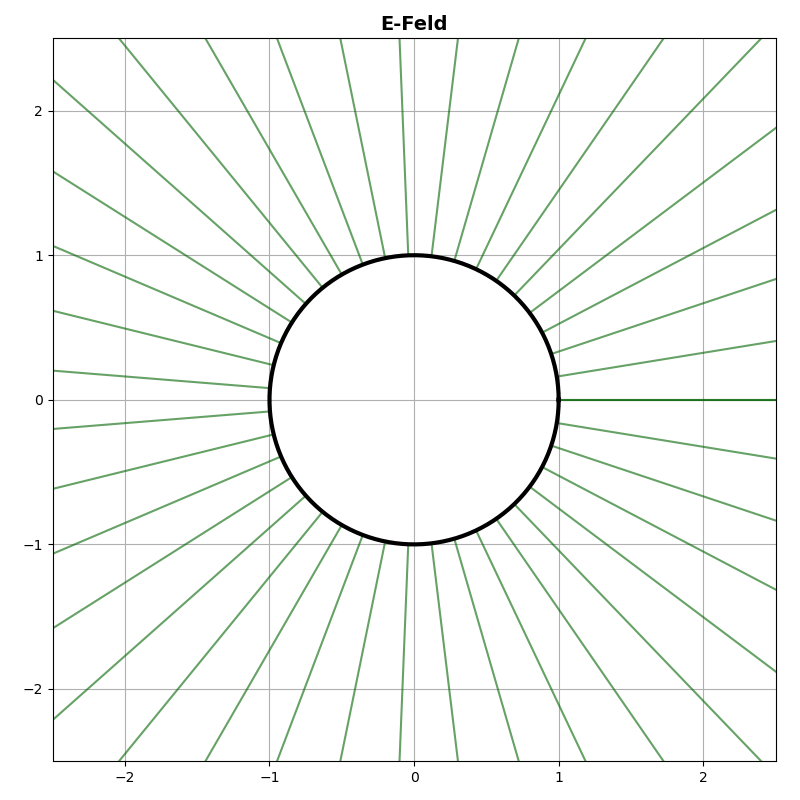
\includegraphics[width=0.9\linewidth]{papers/elektro/grafik/e_feld_kreis.png}
	\label{elektro:figure:e_feld}
	\caption[]{Normiert auf eine Punktladung q handelt es sich beim elektrischen Feld um ein Radialfeld.}
\end{figure}
verwandt.
Bringt man eine Probeladung $q$ in die Nähe einer Punktladung $Q$, so ist die Kraft, welche auf die Probeladung wirkt, als elektrische Feldstärke definiert.
Die Kraft ist das gesamte vektorielle Kraftfeld, das an der jeweiligen Stelle auf $q$ wirkt, und wird in Volt pro Meter angegeben $[\vec{E}] = V/m$.
Es handelt sich um ein Radialfeld (ausgehend von der positiven und führend zur negativen Quelle).

\subsection{Das elektrische Potential $\varphi$
\label{elektro:subsection:Potential}}
Genau wie beim $\vec{E}$-Feld, das durch Normalisierung der Coulomb-Kraft mit einer Probeladung definiert wird, ist das elektrische Potential wie folgt
\begin{equation}
	\varphi = \frac{W}{q} = \frac{Q}{4\pi\varepsilon_0r} = - \int_{\text{Pref}}^P \vec{E} \cdot d\vec{l}
	\label{elektro:equation:Potential}
\end{equation}
durch Normalisierung der Energie $W$ mit einer Probeladung definiert.

Die Einheit von $\varphi$ ist Volt $[\varphi] = V$, und ist wie am Anfang erwähnt ein Skalarfeld.
Somit ist jedem Punkt ein Betrag zugeordnet, und mit Beträgen kann eine Differenz zwischen zwei Punkten im Skalarfeld gebildet werden.
Diese Differenz zwischen zwei Potentialen ist die Spannung, es wird dabei oft ein Referenzpunkt gewählt, der als Nullpunkt dient.
%Aus dem Potential jedes einzelnen Punktes kann die elektrische Feldstärke berechnet werden.
Das negative Vorzeichen in der Formel \eqref{elektro:equation:Potential} hat seinen Ursprung in der Wahl des Bezugssystem, der Referenz Ref, von wo aus integriert wird.
In der Formel \ref{elektro:equation:Potential} wird der Betrag des elektrostatischen Felds $E$ als Variable verwendet, das an jedem Punkt von $E$ auf das dort herrschende Potential geschlossen werden kann und umgekehrt. 
Wenn auf zwei nebeneinanderliegenden Punkten dasselbe Potential $\varphi$ herrscht, werden diese mit einer Linie verbunden, der sogenannten Äquipotentiallinie.
Diese Linien sind immer geschlossen und verlaufen senkrecht zu den E-Feldlinien.
Sie haben aber noch eine weitere wichtige Eigenschaft:
Auf diesen Linien kann eine Probeladung beliebig verschoben werden, ohne dass dabei Arbeit aufgewandt werden muss.
\begin{figure}
	\centering
	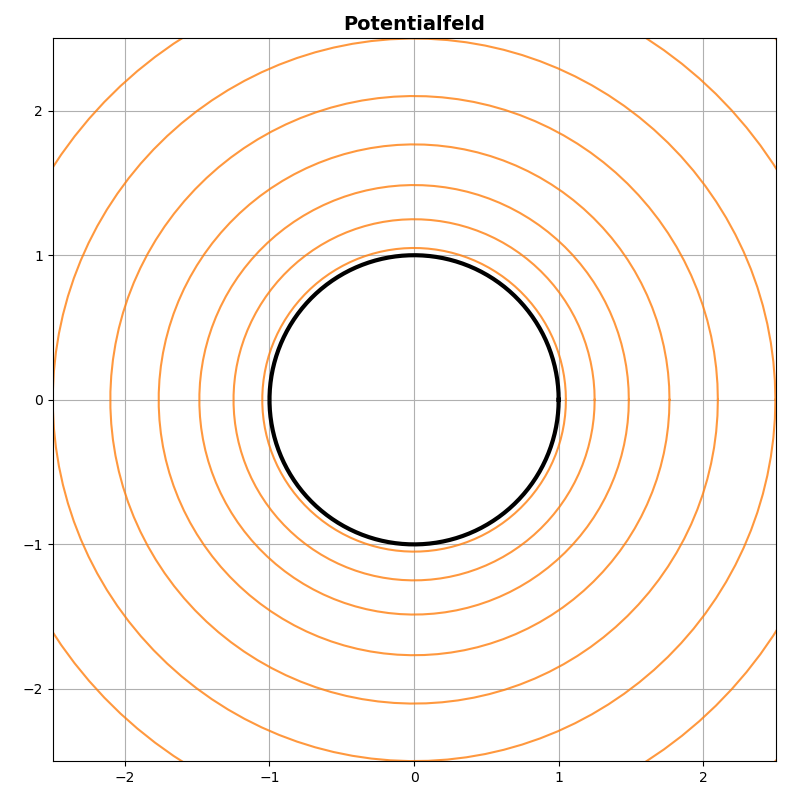
\includegraphics[width=0.9\linewidth]{papers/elektro/grafik/phi_feld_kreis.png}
	\label{elektro:figure:phi_feld}
	\caption[]{Es werden die Äquipotentiallinien dargestellt, um so näher die Linien beieinander liegen, desto höher ist das Potential, und somit auch das elektrische Feld. Der Rand des Kreises hat dabei ein beliebiges Potential gesetzt.}
\end{figure}


%\subsection{Äquipotentiallinien
%\label{elektro:subsection:Aequipotentiallinien}}
%Wie bereits erwähnt, sind die Äquipotentiallinien die Linien, auf denen das Potential $\varphi$ konstant ist.


% \subsection{Beispiel Einheitskreis
% \label{elektro:subsection:Einheitskreis-Beispiel}}
% In den Grafiken \ref{elektro:figure:e_feld} und \ref{elektro:figure:phi_feld} sind die Feldlinien und Äquipotentiallinien dargestellt ausserhalb des Einheitskreises.
% Der Rand des EInheitskreises wird in diesem Kapitel einfach als abgrenzung eines objekts angenommen.
% Das Feld ausserhalb ist dabei immer gleich egal wie hoch das potential ist oder ob einfach nur angenommen wird das der Einheitskreis als einzelne ladung angenommen wird.
% Theoretisch kann angenommen werden das der Kreis auf die Grösse eines Elektrons geschrumpft wird dabei würde das Feld immer noch gleich aussehen. 

\subsection{Zusammenhang zwischen E-Feld und Potential über komplexe Funktionen
\label{elektro:subsection:komplex}}
Das Ziel dieses Abschnitts ist, die Beziehung zwischen Äquipotentiallinien und dem elektrische Feld zu zeigen.
Die beiden Funktionen $\vec{E}$ und $\varphi$ können gemeinsam dargestellt werden.
Dabei wird ein wichtiger Zusammenhang klar: Die Potentiallinien und E-Feldlinien stehen immer senkrecht aufeinander.
Dies wird hier mit komplexen Funktionen erklärt, die in Kapitel \ref{chapter:holomorph} eingeführt wurden.
Dort werden auch die Cauchy-Riemann Gleichungen beschrieben, welche die Grundlage für die Beziehung zwischen den beiden Feldern bilden.
Wir bilden eine komplexe Funktion $f(z) = u(x,y) + iv(x,y)$, hierbei hängen Real- und Imaginärteil nur von den reellen Variablen x und y ab, also den zweidimensionalen Koordinaten unseres Abbildungssystems.
Der Realteil $u$ wird als elektrostatisches Feld definiert und ist nun eine Funktion von $x$ und $y$.
Der Imaginärteil $v$ ist das Potentialfeld.
Beide Funktionen erfüllen die Cauchy-Riemann Gleichungen, und sind daher holomorph. 
Es kann jetzt auch gezeigt werden, wieso die beiden Felder senkrecht aufeinander stehen.
Da diese Funktionen die Laplace-Gleichung 
\begin{equation}
	\Delta u = 0
	\label{elektro:equation:laplace}
\end{equation}
und 
\begin{equation}
	\Delta v = 0
\end{equation}
erfüllen,
kann, wenn eine der beiden bekannt ist, die jeweils andere Funktion sofort bestimmt werden.
Wenn zum Beispiel die Funktion $u$ des elektrischen Feldes bekannt ist, können wir schreiben:
\begin{equation}
	dv = \frac{\partial v}{\partial x}dx + \frac{\partial v}{\partial y} dy = 
	-\frac{\partial u}{\partial y}dx + \frac{\partial u}{\partial x}dy
\end{equation}
und diese Gleichung integrieren, um $v$ zu bestimmen.
Die beiden Vektoren
\begin{equation}
	\nabla{u} = \left(\frac{\partial u}{\partial x}, \frac{\partial u}{\partial y} \right)
\end{equation}
und 
\begin{equation}
	\nabla{v} = \left(\frac{\partial v}{\partial x}, \frac{\partial v}{\partial y} \right)
\end{equation}
stehen senkrecht aufeinander, das heisst sie sind normal zu einander:
\begin{equation}
	\vec{u} \cdot \vec{v} = 0.
\end{equation}
Das bedeutet, die beiden Funktionen $u(x,y)$ und $v(x,y)$ sind lokal senkrecht in ihren Schnittpunkten, 
ebenso wie das elektrische Feld und das Potentialfeld.


%\section{Komplexe Funktionen in der Elektrostatik
%\label{elektro:section:Funktionen-komplexer-Var}}
%Zur Erinnerung: Eine komplexe Zahl $z$ wird in kartesischen Koordinaten als Real- und Imaginärteil wie folgt dargestellt: $z = x + iy$.
%Eine komplexe Funktion $f(z) = u + iv$ kann aufgeteilt werden in zwei Funktionen $u = u(x,y)$ und $v = v(x,y)$, die von den realen Variablen $x$ und $y$ abhängig sind.
%Ein erstes Beispiel ist die Funktion $f(z) = z^{2}$.
%Da mit den Real- und Imaginärteilen wie gewohnt gerechnet werden kann, ergibt das Quadrieren: 
%\begin{equation}
%	(x+iy)^{2} = x^{2} - y^{2} + i2xy,
%\end{equation} 
%mit
%\begin{equation}
%	u(x,y) = x^{2} - y^{2}
%\end{equation} 
%und 
%\begin{equation}
%	v(x,y) = 2xy.
%\end{equation}

%\subsection{Holomorphe oder analytische Funktion
%\label{elektro:subsection:holomorph}}
%Die kontinuierlichen Funktionen $u(x,y)$ und $v(x,y)$ mit kontinuierlichen partiellen Ableitungen sind dann holomorph, wenn sie die Cauchy-Riemann Gleichungen
%\begin{equation}
%	\label{elektro:subsection:holomorph:Cauchy1}
%	\frac{\partial u}{\partial x} = \frac{\partial v}{\partial y}
%\end{equation}
%und 
%\begin{equation}
%\label{elektro:subsection:holomorph:Cauchy2}
%	\frac{\partial u}{\partial y} =
%	- \frac{\partial v}{\partial x}
%\end{equation}
%
%erfüllen.
%Holomorph bedeutet differenzierbar in jeder Ordnung und darstellbar als Exponentialreihe.
%Das Integral der Funktion entlang eines geschlossenen Weges in der komplexen Zahlenebene ist Null
%\begin{equation}
%	\oint f(z) \,dz = 0.
%\end{equation}
%\textcolor{red}{Streichen, auf Kapitel 1 und 2 verweisen}


%\subsection{Gausssches Gesetz
%\label{elektro:subsection:Gauss}}



%\subsection{Zusammenhang zwischen E-Feld und Potential
%\label{elektro:subsection:ephizusammenhang}}
%Etwas vorgreifend wird hier gezeigt, wie im Falle eines Kreises mathematisch von einem Potentialfeld $\varphi$ auf das elektrische Feld $\mathbf{E}$ geschlossen werden kann.
%Die Fläche außerhalb des Kreises wird als Potentialfeld beschrieben.
